\chapter[Estrutura]{Estrutura organizacional da instituição estudada} \label{chap:instituicao}

Para que se possa entender melhor o problema, é necessário que se entenda a estrutura organizacional da \LinkToURL{\LinkSiteUENF}{Universidade Estadual do Norte Fluminense Darcy Ribeiro (UENF)} disposta no Estatuto da UENF (\cite{Estatuto2002}), ainda que limitado ao que convém ao escopo deste trabalho.

\section{A UENF e seu estatuto} % ### 4.1. A UENF e seu estatuto     % Adicionar links corretos nos laboratórios e centros

% Provavelmente eu deveria adicionar informações sobre a secretaria acadêmica
% Precisa de revisão
% Sinto que falta falar sobre secretaria acadêmica e Conselho de Centro

Segundo o estatuto, a UENF compreende:

\begin{itemize}
  \item Órgãos da Administração Superior de política, gestão e supervisão;
  \item Unidades universitárias de ensino, pesquisa e extensão;
  \item Órgãos e serviços especiais, destinados a auxiliar na administração e a suplementar as atividades de ensino, pesquisa, extensão e apoio técnico.
\end{itemize}

% - Órgãos da Administração Superior de política, gestão e supervisão;
% - Unidades universitárias de ensino, pesquisa e extensão;
% - Órgãos e serviços especiais, destinados a auxiliar na administração e a suplementar as atividades de ensino, pesquisa, extensão e apoio técnico.

Quanto aos órgãos da Administração Superior devemos enfocar o órgão executivo, constituído unicamente pela reitoria, cujos órgãos auxiliares englobam a Secretaria Acadêmica, que por sua vez tem como algumas de suas atribuições as seguintes:

\begin{enumerate}
  \item Coordenar a \textbf{divulgação do horário escolar dos vários cursos da UENF}, de modo a \textbf{otimizar os recursos humanos}, \textbf{ampliar as opções de disciplinas para os alunos} e tornar acessíveis os dados escolares;
  \item \textbf{Centralizar os serviços de registro da vida escolar dos alunos}, compreendendo \textbf{inscrição}, admissão, \textbf{matrícula}, \textbf{créditos}, \textbf{opções}, transferências, promoções, graduações e preparação dos respectivos diplomas, dentro das normas estabelecidas.
\end{enumerate}

Já quanto as unidades universitárias de ensino, temos no estatuto que ``as unidades universitárias de ensino, pesquisa e extensão, definidas por áreas de conhecimento, são constituídas em Centros, que por sua vez congregam Laboratórios afins'' e que ``o Laboratório é a menor parte da estrutura universitária para todos os efeitos de organização administrativa, didático-científica, distribuição de pessoal e de representação nos órgãos colegiados da UENF''.

A administração do Centro é da competência do Diretor e seu Conselho. Os Laboratórios, por sua vez, são administrados pelos Chefes de Laboratório.

O Conselho de Centro, tem como uma de suas atribuições, descrito no inciso XVII do artigo 34 do estatuto, a seguinte: \textbf{designar, semestralmente, os professores responsáveis pelas disciplinas dos Cursos de Graduação} e Programas de Pós-Graduação, ouvidos os respectivos Laboratórios, os Colegiados de Curso e Comissões de Coordenação.

Atualmente, segundo o site da UENF, a universidade possui 4 Centros, sendo eles:

\begin{enumerate}
  \item Centro de Ciências do Homem - \LinkToURL{\LinkCCH}{CCH};
  \item Centro de Ciência e Tecnologia - \LinkToURL{\LinkCCT}{CCT};
  \item Centro de Biociências e Biotecnologia - \LinkToURL{\LinkCBB}{CBB};
  \item Centro de Ciências e Tecnologias Agropecuárias - \LinkToURL{\LinkCCTA}{CCTA}.
\end{enumerate}

E também existem 8 \LinkToURL{\LinkLaboratorios}{laboratórios} vinculados ao Centro de Ciência e Tecnologia (CCT), sendo eles:

\begin{enumerate}
  \item Laboratório de Meteorologia – \LinkToURL{\LinkLAMET}{LAMET};
  \item Laboratório de Ciências Físicas – \LinkToURL{\LinkLCFIS}{LCFIS};
  \item Laboratório de Engenharia Civil – \LinkToURL{\LinkLECIV}{LECIV};
  \item Laboratório de Ciências Químicas – \LinkToURL{\LinkLCQUI}{LCQUI};
  \item Laboratório de Materiais Avançados – \LinkToURL{\LinkLAMAV}{LAMAV};
  \item Laboratório de Ciências Matemáticas – \LinkToURL{\LinkLCMAT}{LCMAT};
  \item Laboratório de Engenharia de Produção – \LinkToURL{\LinkLEPROD}{LEPROD};
  \item Laboratório de Engenharia e Exploração de Petróleo – \LinkToURL{\LinkLENEP}{LENEP}.
\end{enumerate}

Os Laboratórios englobam os Cursos de Graduação e Pós-Graduação, que são administrados pelos Coordenadores de Curso.

Além disso, o LCMAT mantém dois cursos de graduação e um programa de pós-graduação stricto sensu. Sendo eles:

\begin{enumerate}
  \item \LinkToURL{\LinkLicMat}{Licenciatura em Matemática};
  \item \LinkToURL{\LinkSiteCCUENF}{Bacharelado em Ciência da Computação};
  \item \LinkToURL{\LinkLCMATPósGraduação}{Mestrado Profissional em Matemática} – \LinkToURL{\LinkUENFPósGraduações}{PROFMAT} / \LinkToURL{\LinkProfMat}{SBM}.
\end{enumerate}

\section{Entrevistas} \label{sec:entrevistas} % ### 4.2.

% Separar entrevists de minhas opiniões pessoais

Como forma de entender melhor a percepção real daqueles que recorrentemente lidam com a tarefa de criação da grade horária, diversas entrevistas foram feitas com o intuito de analisar qualitativamente quais são as opiniões, pedidos, reclamações e pensamentos de diferentes níveis organizacionais da UENF.

\subsection{Diretor do CCT} % #### 4.2.1. Diretor do CCT

% Devo omitir o nome dos entrevistados?

O primeiro entrevistado foi o atual Diretor do CCT. Ele atualmente estrutura a relação de disciplinas ofertadas pelo CCT em Excel e as publica \LinkToURL{\LinkDistribuiçãoDeSalas}{em formato PDF no site do CCT}. Seu trabalho auxilia os Chefes de Laboratório e Coordenadores de Curso a visualizarem quais são as salas disponíveis e em quais horários cada professor está alocado.

Um dos tópicos dialogados, foi quanto às categorias das disciplinas, ou seja, quais características notáveis as disciplinas poderiam ter. Com isso podemos listar as seguintes categorias de disciplinas:

\begin{itemize}
  \item \textbf{Anuais}: disciplinas que ocorrem apenas uma vez no ano;
  \item \textbf{Ímpares}: disciplinas que são ofertadas no primeiro semestre letivo;
  \item \textbf{Pares}: disciplinas que são ofertadas no segundo semestre letivo;
  \item \textbf{De serviço}: disciplinas ofertadas para mais de um curso simultaneamente;
  \item \textbf{Ciclo básico}: disciplinas oferecidas para todas as engenharias;
  \item \textbf{Repetentes}: turmas criadas especialmente para repetentes.
\end{itemize}

% - Anuais: disciplinas que ocorrem apenas uma vez no ano;
% - Ímpares: disciplinas que são ofertadas no primeiro semestre letivo;
% - Pares: disciplinas que são ofertadas no segundo semestre letivo;
% - De serviço: disciplinas ofertadas para mais de um curso simultaneamente;
% - Ciclo básico: disciplinas oferecidas para todas as engenharias;
% - Repetentes: turmas criadas especialmente para repetentes.

As disciplinas ímpares e pares geralmente estão atreladas à expectativa de que os alunos progredirão sequencialmente sem reprovação alguma. Entretanto, caso uma quantidade de alunos considerável de alunos reprove em determinada disciplina, é possível que estes se enquadrem na criação de uma turma especial para repetentes, ou não.

Uma sugestão de utilidade para o software é a de permitir que as ``disciplinas de serviço'' sejam fixas, visto que estas são as que têm maior complexidade de manejamento de horário posteriormente, justamente por geralmente abrangerem muitos alunos e de diversos cursos diferentes.

Uma outra característica notável é a repetição de atribuições de disciplinas em pares regulares, ou seja, alocadas no mesmo período de horário com um dia de intervalo entre elas. Um exemplo desse tipo de alocação recorrente seria ``14 às 16 horas de segunda e quarta feira''.

Com isso, surge a dúvida: há uma preferência ativa por aulas alocadas com este padrão? A resposta dada é que não. O que se mostra como uma restrição a menos na hora de se alocar as turmas.

Outro caso notável é a existência majoritárias de turmas criadas com dois períodos de duas horas, entretanto existem algumas que fogem deste padrão e possuem três horas de duração. A solução encontrada pelo Diretor é a de colocar esta disciplina começando às 10h, o que faz com que se alongue até as 13h, período geralmente usado pelos estudantes e servidores para se alimentar, e justamente por isso evitando que atrapalhe a distribuição das salas. Outra alternativa é alocar esta turma para as 13h, fazendo com que finalize às 16h, horário em que as disciplinas com duas horas de duração geralmente terminam.

Segundo ele, saber a demanda máxima possível seria bom, visto que podem haver casos de solicitações de vagas para disciplinas de serviço que extrapolam a quantidade esperada para a distribuição balanceada dentre os cursos.

Uma outra situação que ocorre é que algumas disciplinas historicamente têm seus horários definidos em um mesmo horário ao longo dos anos. Caso essa alocação seja alterada, ocorre a possibilidade de reclamação por parte dos professores, mesmo que esta alteração seja benéfica para os estudantes. Então por exemplo, os horários de 8h de uma segunda feira e de 16h de sexta feira, não são geralmente desejados pelos professores, mesmo que eles teoricamente tenham disponibilidade de 8 horas diárias.

Considerando a quantidade de laboratórios ``concorrendo'' simultaneamente às vagas, surge a dúvida: há ordem de precedência entre os laboratórios? A resposta para esta pergunta é ``Não. As vagas são distribuídas com prioridade na ordem de chegada''.

Algumas outras informações que ele elenca:

\begin{itemize}
  % \item Os períodos ímpares são os piores;
  % \item Essa opinião pode ser resultado do fato de que os períodos ímpares apresentam um intervalo de tempo para preparo das grades menor do que os períodos pares;
  % Comentei porque não faz sentido. As que têm menos tempo são os períodos pares.
  \item \textbf{As disciplinas básicas são grandes}: é esperado que uma grande quantidade de alunos se inscreva nas disciplinas essenciais e iniciais de seus cursos, sendo boa parte dela relacionada com o conceito das disciplinas de serviço e com o conceito de ciclo básico das engenharias;
  \item \textbf{As disciplinas de serviço devem ser alocadas primeiro}: visto a grande quantidade de conflitos possíveis dentre os diversos cursos, ao alocá-las primeiro, os conflitos passam a ocorrer em turmas com uma quantidade menor de pessoas e/ou que sejam de um mesmo curso;
  \item \textbf{As alterações vão até o final do período}: embora possa parecer que a alocação de turmas finalize após o encerramento do período de inscrição e desinscrição, na prática,a realocação ocorre durante todo o período;
  \item \textbf{Teoricamente matérias de um mesmo período não devem conflitar}: isso se dá segundo a percepção de que a maioria dos alunos está seguindo a mesma linha sequencial de disciplinas, o que muitas das vezes não é a realidade.
\end{itemize}

\subsection{Desenvolvedor do Sistema Acadêmico} % #### 4.2.2. Desenvolvedor do Sistema Acadêmico

Considerando que a integração do sistema proposto seria certamente mais eficiente se integrada ao sistema acadêmico, viu-se como apropriado entrevistar o desenvolvedor do Sistema Acadêmico para se ponderar sobre o uso dos dados e a possível integração.

Durante a entrevista, foram listados alguns dados que seriam interessantes para a análise, sendo eles a demanda de disciplinas, a listagem dos professores, a listagem dos alunos aprovados e suas respectivas disciplinas e por fim os requisitos das disciplinas.

% - Demanda de disciplinas
% - Listagem de professores
% - Listagem dos alunos aprovados
% - Requisitos das disciplinas

Outra questão analisada seria quanto a forma de integração. Boa parte das aplicações web se comunicam em forma de API, entretanto, devido à quantidade de alterações executadas ao longo do semestre no sistema acadêmico, o Desenvolvedor do Sistema Acadêmico utiliza o sistema de mensagerias através do \LinkToURL{\LinkRabbitMQ}{RabbitMQ}.

Foi citado sobre a abordagem do Coordenador de Computação para o cálculo das demandas, quanto a isso, o Desenvolvedor citou que poderia facilmente permitir o download de um CSV dos dados necessários.

Quanto à possibilidade de aprimoramentos no Sistema Acadêmico, ele disse que ``eu faço o que me pedem'', se referindo ao repositório do Acadêmico disponível no \LinkToURL{\LinkGitLab}{GitLab}, onde alguns poucos usuários fazem solicitações de alterações e melhorias. Havendo então a possibilidade de que o Coordenador de Computação faça uma solicitação à SECACAD para que seja implementada uma funcionalidade que permita a exportação dos dados necessários para o cálculo das demandas.

Um outro problema apontado por ele é a falta de gente. Segundo ele, outras duas pessoas entraram junto com ele no mesmo concurso, mas foram realocadas para outras áreas da universidade. Ele cita também sobre a ``cultura do trabalho opcional'' existente na UENF, onde muitos servidores não se sentem obrigados a trabalhar.

Em relação a estrutura dos dados, o sistema acadêmico utiliza o SQL. Foi citado o uso de NOSQL e estrutura de Grafos como possibilidades de mudança, mas como a mesma não se mostrou necessária até o momento, não foi implementada.

Uma questão levantada pelo entrevistado diz respeito à manutenção do software desenvolvido neste trabalho. Não sabendo ele dizer se o mesmo seria mantido pela UENF.

Ele também sugere que, para evitar a complexidade de se trabalhar com dados reais de alunos, que sejam utilizados dados fictícios.

\subsection{Chefe de Laboratório de Matemática} % #### 4.2.3. Chefe de Laboratório de Matemática

Considerando que um dos cargos relacionados com o processo de elaboração de grades horários é o de Chefe de Laboratório, foi entrevistada a atual Chefe de Laboratório de Matemática.

Assim como sugerido pelo Desenvolvedor do Sistema Acadêmico, a Chefe também sugeriu que dados fictícios fossem utilizados. Sugeriu ainda que fosse utilizado o schema do banco de dados do sistema acadêmico como sua criação. Outra sugestão foi a solicitação ao Desenvolvedor do Sistema Acadêmico uma listagem de possíveis valores recorrentes no banco de dados.

A entrevistada também relatou algumas problemáticas envolvendo a realocação dos horários das turmas. Segundo ela, qualquer alteração pode ser feita durante a semana anterior à matrícula, visto que, não havendo inscritos, não há problema na alteração. A partir do momento em que houver ao menos um aluno inscrito na disciplina, alterações só podem ser feitas caso não haja conflitos aparentes e preferencialmente com um documento assinado pelos alunos que estiverem inscritos.

\subsection{Responsável pela Secretaria Acadêmica (SECACAD)} % #### 4.2.4. Responsável pela Secretaria Acadêmica (SECACAD)

Inicialmente, alguns tópicos foram trazidos como ponto focal da entrevista, sendo alguns deles os seguintes:

\begin{itemize}
  \item Dúvidas quanto as atribuições da SECACAD;
  \item Permissão de acesso aos dados que não são estritamente necessários, mas ajudariam;
  \item Definição dos períodos, demanda provisória e erros de estimativa;
  \item GitLab, tarefas (issues) e demandas;
  \item Automatização da burocracia;
  \item Ética VS Eficiência.
\end{itemize}

% - Dúvidas quanto as atribuições da SECACAD
% - Permissão de acesso aos dados que não são estritamente necessários, mas ajudariam
% - Definição dos períodos, demanda provisória e erros de estimativa
% - GitLab, tarefas (issues) e demandas
% - Automatização da burocracia
% - Ética VS Eficiência

Logo de início, o entrevistado informou que ele não pode ceder dados de nenhum aluno, mesmo que anonimizados, mas sugeriu que poderia reencaminhar um formulário de pesquisa para os alunos, para que assim eles próprios pudessem fornecer os dados necessários.

Outra abordagem interessante informada por ele é quanto ao seu conhecimento técnico, onde sugeriu abordagens de análise multicritérios como forma de se auxiliar a criação das grades horárias.

Durante a conversa, foi citado de forma positiva quanto à demanda exata de cada disciplina. Reforçou-se a preferência pela alocação de disciplinas visando os estudantes mais próximos da conclusão do curso, estando em último na ordem de prioridade aqueles que decidem se adiantar com disciplinas de períodos mais avançados. Uma outra característica apontada é que a sequência de definições é a seguinte: Vagas $\rightarrow$ Professor $\rightarrow$ Sala $\rightarrow$ Horário.

Também se confirmou a não existência de um registro oficial das salas e suas capacidades. Essa informação é inserida como um campo de texto no sistema acadêmico, com isso, o sistema não impediria a alocação de duas turmas em uma mesma sala em um mesmo horário.

O responsável pela SECACAD também informou que cabe à Pró-Reitoria a mudança do início do primeiro semestre para expandir o período de preparação das grades horárias para o segundo período, sendo que este pedido deve partir da Câmara de Graduação.

Quanto ao tópico ``ética VS eficiência'', ele citou que embora o sistema acadêmico impeça a realocação de turmas com alunos inscritos, é possível que o mesmo seja burlado ao manualmente se excluir a inscrição do aluno. Sendo esta prática justificável em alguns casos.

Uma ferramenta que o beneficiaria seria a análise dos alunos que estão à beira de perder o vínculo com a universidade, para que a Secretaria Acadêmica possa tomar as medidas cabíveis.

\subsection{Coordenador de Computação} % #### 4.2.5. Coordenador de Computação

Sendo o Coordenador de Computação o principal usuário do sistema, torna-se imprescindível a análise qualitativa de sua perspectiva.

Seguindo o conceito de Design Iterativo utilizado também por \citeonline{Andre2018}, o Coordenador foi consultado em diversas etapas do desenvolvimento do sistema. Inicialmente, foi apresentado a ele o conceito do sistema, suas funcionalidades e possíveis benefícios. Em seguida, foi apresentado a ele um protótipo do sistema. Mas esta questão será melhor tratada em outro segmento deste mesmo trabalho, aqui será abordado apenas o conteúdo das entrevistas.

Assim como comentado pelo Diretor do CCT, o Coordenador também fala sobre a definição de matérias que se mostram fixas, porém, agora com outro olhar: enquanto o diretor vê as matérias fixas como uma forma de atribuição histórica seguindo a ideia de ``já era assim quando eu cheguei'', o Coordenador por sua vez vê apenas como uma forma predefinida e imutável. Porém, olhando em um contexto mais amplo, essa definição de matérias não se mostra como obrigatória, visto que pode haver casos em que outra alocação de uma disciplina ``fixa'' apresente uma qualidade melhor do que seu horário usual.

Outra questão levantada por ele é quanto a um problema já antigo no curso de Ciência da Computação na UENF, que há anos apresenta um corpo docente reduzido em comparação com outros cursos, sendo necessário um desdobramento maior para suprir a demanda de disciplinas dos alunos. Uma solução utilizada é a de solicitar a abertura de uma bolsa para docência complementar, onde um aluno de pós-graduação pode ser alocado como professor de uma disciplina. Solução que embora não seja a ideal, é a que se mostra mais viável, dada a diminuta inscrição de candidatos à docência.

Uma outra característica até então não citada pelos outros entrevistados é que existem salas que são vistas culturalmente como sendo de determinado curso, onde acaba sendo um certo tabu a alocação de uma disciplina de outro curso, mesmo que não se esteja infringindo regra alguma.

Quanto à priorização de veteranos já citada anteriormente, o Coordenador aponta uma outra forma de se enxergar a situação: em disciplinas dos períodos finais do curso, a prioridade é dos veteranos, ficando os calouros que ocasionalmente possam ter se adiantado, em segundo plano. Já em disciplinas dos períodos iniciais, a prioridade é dos calouros, ficando os veteranos que por ventura tenham reprovado, em segundo plano.

Diferente de como foi respondido pelo Diretor do CCT, para o Coordenador de Computação a alocação de disciplinas em pares se mostra como ``didática'', sendo ela então preferível, mas não necessariamente vista como obrigatória.

Considerando a recorrência de citação do conceito de estimativas de demanda, o Coordenador de Computação sugere que haja um campo no sistema para que seja inserida a demanda estimada de cada disciplina.

Considerando que no contexto atual do curso de Ciência da Computação na UENF é iminente a adoção de uma nova grade curricular, o Coordenador apresentou preocupação em relação à possibilidade de que o sistema não seja mais utilizado após a adoção da nova grade. Essa questão encontra-se atualmente fora do escopo do atual projeto, entretanto, não se mostra como um problema de difícil solução, visto que o sistema pode ser adaptado para a nova grade.

\subsection{Entendimento geral das entrevistas} % #### 4.2.6. Entendimento geral das entrevistas

Podemos concluir após a análise qualitativa das entrevistas que há de fato um certo grau de insatisfação por parte dos usuários do sistema atual. Embora o sistema funcione, ele apresenta gargalos que poderiam ser resolvidos com a utilização de um sistema mais eficiente que envolvesse mais diferente as diferentes partes interessadas. Suas maiores insatisfações são quanto à burocracia e o curto período de tempo disposto para a elaboração das grades horárias.

Embora não sejam apontadas como insatisfação, algumas potenciais ferramentas e melhorias foram também citadas pelos entrevistados. Dentre elas, a demanda máxima possível, que passaria a evitar superestimações de demanda, a alocação de disciplinas de serviço como fixas, e em alguns casos, a alocação de disciplinas em pares, que embora não seja uma regra, é uma preferência de um dos entrevistados. Outra ferramenta que foi citada é a de análise de alunos à beira de perder o vínculo com a universidade, que poderia ser utilizada pela Secretaria Acadêmica para tomar as medidas cabíveis. Também se fazendo notória a necessidade de registro oficial das salas e suas capacidades, que atualmente é inserida como um campo de texto no sistema acadêmico.

Outros problemas encontrados, remetem à acomodação institucional de algumas práticas, como a alocação de disciplinas em horários fixos, em pares e/ou nas mesmas salas. Essas práticas, embora não sejam obrigatórias, são vistas como um costume e por isso são mantidas.

\section{Sequência de criação das grades horárias} % ### 4.3.

% Estou com dúvida novamente de qual é a progressão e de quem faz o quê

Ao somarmos o conhecimento presente no estatuto da UENF, com o conhecimento adquirido através das entrevistas, podemos ter uma visão geral de como se dá a criação das grades horárias na UENF. Assim, abaixo estão listados os passos que geralmente são seguidos para a criação das grades horárias.

% Fazer um diagrama de... sei lá, aquele que tem barras retas. Diagrama de atividades?

\begin{enumerate}
  \item Período ocorrendo normalmente;
  \item Coordenadores enviam para Chefes de Laboratório uma demanda estimada de cada uma das disciplinas que serão ofertadas;
  \item Chefes de Laboratório atrelam professores a disciplinas;
  \item Chefes de Laboratório enviam para Diretores de Centro a demanda estimada;
  \item Dependendo das disponibilidades dos professores, cabe solicitar a abertura de uma bolsa de apoio ao ensino;
  \item O Diretor aloca provisoriamente as disciplinas em horários e salas;
  \item O Coordenador de Curso analisa possíveis mudanças de horários que possam ser mais eficientes na distribuição dos alunos;
  \item O período letivo acaba;
  \item Estima-se mais precisamente a demanda de cada disciplina;
  \item Turmas são abertas com a quantidade de vagas de acordo com as demandas estimadas;
  \item Alunos se inscrevem;
  \item Últimas mudanças são feitas;
  \item Período de inclusão e exclusão;
  \item Alguns possíveis ajustes finais;
  \item Período ocorrendo normalmente.
\end{enumerate}

% 1. Período ocorrendo normalmente;
% 2. Coordenadores enviam para Chefes de Laboratório uma demanda estimada de cada uma das disciplinas que serão ofertadas;
% 3. Chefes de Laboratório atrelam professores a disciplinas;
% 4. Chefes de Laboratório enviam para Diretores de Centro a demanda estimada;
% 5. Dependendo das disponibilidades dos professores, cabe solicitar a abertura de uma bolsa de apoio ao ensino;
% 6. O Diretor aloca provisoriamente as disciplinas em horários e salas;
% 7. O Coordenador de Curso analisa possíveis mudanças de horários que possam ser mais eficientes na distribuição dos alunos;
% 8. O período letivo acaba;
% 9. Estima-se mais precisamente a demanda de cada disciplina;
% 10. Turmas são abertas com a quantidade de vagas de acordo com as demandas estimadas;
% 11. Alunos se inscrevem;
% 12. Últimas mudanças são feitas;
% 13. Período de inclusão e exclusão;
% 14. Alguns possíveis ajustes finais;
% 15. Período ocorrendo normalmente.

Entrando em detalhes ainda maiores, podemos citar uma das etapas de criação das grades horárias que é a coleta de uma demanda esperada. Nela, cada Coordenador elabora de seu próprio modo. Uma possibilidade seria analisar quantos alunos costumam reprovar em determinada disciplina pela visualização estatística anterior, somado aos que possivelmente aprovarão na disciplina que é pré-requisito. Porém, toda essa pesquisa e estimativa é dispendiosa e pode desagradar a alguns coordenadores, ou então gerar estimativas incondizentes com a realidade.

Entendemos então que dentro do contexto da universidade, o problema de agendamento se torna mais complexo pois um dos recursos que está relacionado com o problema é a existência de prazos em cada uma das etapas, assim fazendo com que uma solução ideal seja aquela que é capaz de ser executada dentro do prazo estipulado, mesmo que não seja ótima.

\section{Formulário de pesquisa} % ### 4.4. Formulário de pesquisa % Adicionar as imagens do formulário

% CORRIGIR FUTURAMENTE - XXX Checar se as perguntas nas tabelas, prints e anexo são as mesmas

Como forma de analisar também a perspectiva dos discentes quanto à problemática abordada, foi elaborado um formulário de pesquisa com o intuito de se confirmar ou não a hipótese de que em sua maioria os alunos também se encontram insatisfeitos com a atual conjuntura de distribuição e alocação de turmas.

Para este fim, foi utilizado um formulário de pesquisa qualitativa dos alunos disponível no Apêndice 1. O formulário foi divulgado através de um link disponibilizado no grupo de alunos do curso de Ciência da Computação no WhatsApp, e também através de um link distribuído pela Secretaria Acadêmica a discentes da UENF.

A seguir, estão dispostos alguns resultados obtidos pelo formulário.

\subsection{Respondentes} % #### 4.4.1. Respondentes

Inicialmente foi solicitadas algumas informações dos alunos, como seu curso, ano de ingresso. As respostas estão dispostas na \autoref{fig:2.0-SobreVoce}.

\begin{MyCenteredFigure}
  \caption{Perguntas sobre o curso e ano de ingresso dos estudantes}
  \label{fig:2.0-SobreVoce}
  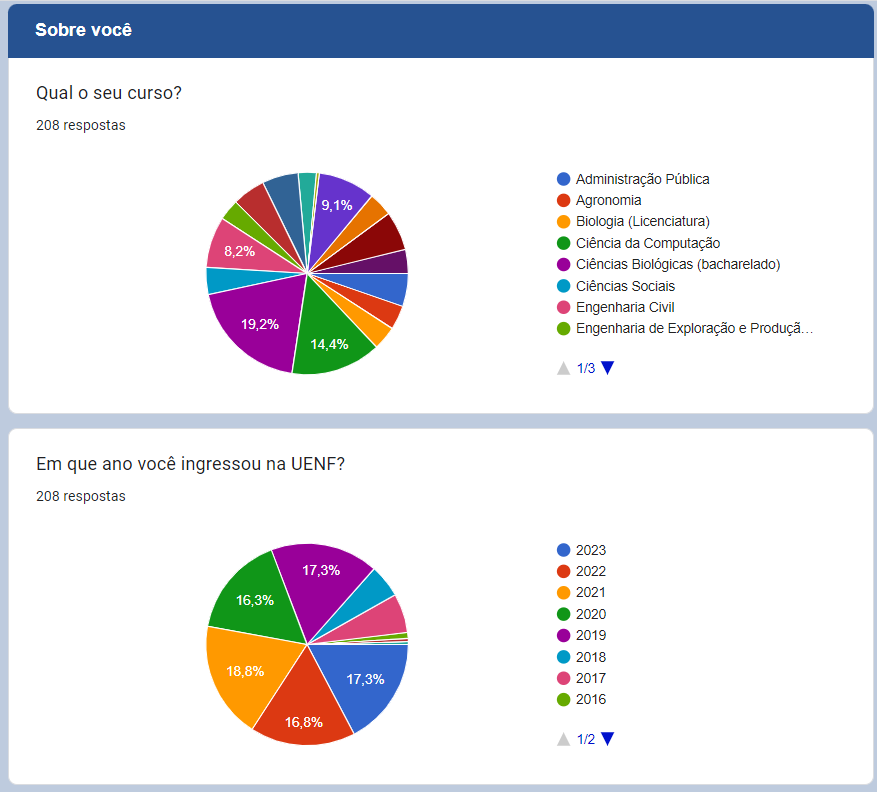
\includegraphics[width=\textwidth]{files/img/2.02!3-organizacao/2.02!3.1.4-forms/2.0-SobreVoce}
\end{MyCenteredFigure} % SobreVoce

O formulário foi respondido por 208 alunos, sendo os cursos de maior incidência o bacharelado de Ciências Biológicas com 40 respondentes, Ciência da Computação com 29 e Medicina Veterinária com 19 (\autoref{table:2.1_SobreVoce_Cursos}). Vale ressaltar que 96 dos respondentes são alunos de cursos que envolvem diretamente o CCT. Entretanto, a análise dos gráficos abordará a percepção de todos igualmente.

\begin{table}[htbp]\centering
  \caption{Número de respondentes por curso}
  \label{table:2.1_SobreVoce_Cursos}
  \begin{tabular}{| r l |}
    \hline
    \textbf{Quantidade} & \textbf{Curso}                                  \\
    \hline
    40                  & Ciências Biológicas (bacharelado)               \\
    29                  & Ciência da Computação                           \\
    19                  & Medicina Veterinária                            \\
    17                  & Engenharia Civil                                \\
    13                  & Química (Licenciatura)                          \\
    12                  & Engenharia Metalúrgica                          \\
    11                  & Engenharia de Produção                          \\
    11                  & Administração Pública                           \\
    9                   & Ciências Sociais                                \\
    8                   & Agronomia                                       \\
    8                   & Biologia (Licenciatura)                         \\
    8                   & Pedagogia (Licenciatura)                        \\
    8                   & Zootecnia                                       \\
    7                   & Engenharia de Exploração e Produção de Petróleo \\
    6                   & Física (licenciatura)                           \\
    1                   & Matemática (Licenciatura)                       \\
    0                   & Engenharia Meteorológica                        \\
    0                   & Outro                                           \\
    \hline
  \end{tabular}
\end{table}

Vemos também a distribuição dos anos de ingresso dos alunos que responderam o formulário, sendo seu quantitativo bem distribuído entre os anos de 2019 e 2023, tendo os anos de 2017 e 2018 uma quantidade menor de respostas, os outros anos tendo em conjunto um total de 4 respostas (\autoref{table:2.2_SobreVoce_Anos}).

\begin{table}[htbp]\centering
  \caption{Número de respondentes por ano}
  \label{table:2.2_SobreVoce_Anos}
  \begin{tabular}{| c c |}
    \hline
    \textbf{Quantidade} & \textbf{Ano} \\
    \hline
    36                  & 2023         \\
    35                  & 2022         \\
    39                  & 2021         \\
    34                  & 2020         \\
    35                  & 2019         \\
    11                  & 2018         \\
    13                  & 2017         \\
    2                   & 2016         \\
    1                   & 2015         \\
    0                   & 2014         \\
    0                   & 2013         \\
    1                   & Outro        \\
    \hline
  \end{tabular}
\end{table}

\subsection{Avaliação de experiência acadêmica} % #### 4.4.2. Pesquisa de satisfação

Considerando que o escopo deste trabalho revolve em torno da alocação de recursos físicos e humanos, como salas, professores e alunos, foi elaborada uma seção do formulário de pesquisa com o intuito de se analisar a frequência de ocorrência de certas situações no contexto universitário. Para isto, foram feitas as seguintes perguntas:

\begin{enumerate}
  \item Salas: Você já teve que mudar de sala por falta de algum acessório como quadro, projetor ou monitor? % 53.1%
  \item Salas: Você já teve aula cuja sala não dispunha de carteiras o suficiente? % 52.7%
  \item Vagas: Você já quis entrar em uma disciplina, mas ela não tinha vaga? % 85.0%
  \item Vagas: Você já ficou acordado após meia-noite por medo de não ter vaga para as disciplinas que deseja cursar? % 91.3%
  \item Conflitos: Você já deixou de se inscrever em uma disciplina por causa de conflito de horário? % 90.8%
  \item Preferências: Você já preferiu não se inscrever em uma disciplina para cursá-la em outro momento mais oportuno? % 86.0%
  \item Opiniões: Você acha que a universidade deveria oferecer horários diferentes para as disciplinas mais demandadas para evitar conflitos com outras  % 100.0%
\end{enumerate}

A enumeração das perguntas feitas se encontra representada com suas respectivas respostas na \autoref{table:3.0_satisfacao}.

\begin{table}[htbp]\centering
  \caption{Ocorrência de experiências acadêmicas}
  \label{table:3.0_satisfacao}
  \begin{tabular}{| c | c c c |}
    \hline
    \multicolumn{1}{|c|}{\multirow{2}{*}{Pergunta}} & \multicolumn{3}{c|}{Respostas}
    \\
    \multicolumn{1}{|c|}{}                          &
    Sim                                             &
    \multicolumn{1}{|c|}{Não}                       &
    Outro
    \\
    \hline
    1                                               & 110                            & 87 & 10 \\ % 110/207=0.5314 =  53.1%
    2                                               & 109                            & 95 & 3  \\ % 109/207=0.5265 =  52.7%
    3                                               & 176                            & 28 & 3  \\ % 176/207=0.8502 =  85.0%
    4                                               & 189                            & 17 & 1  \\ % 189/207=0.9130 =  91.3%
    5                                               & 188                            & 15 & 4  \\ % 188/207=0.9082 =  90.8%
    6                                               & 178                            & 27 & 2  \\ % 178/207=0.8599 =  86.0%
    7                                               & 207                            & 0  & 0  \\ % 207/207=1.0000 = 100.0%
    \hline
  \end{tabular}
\end{table}

As respostas respectivas às perguntas se encontram na \autoref{fig:3.0_Satisfacao} onde estão dispostos os resultados encontrados nesta seção.

\begin{MyCenteredFigure}
  \caption{Respostas sobre a satisfação dos estudantes}
  \label{fig:3.0_Satisfacao}
  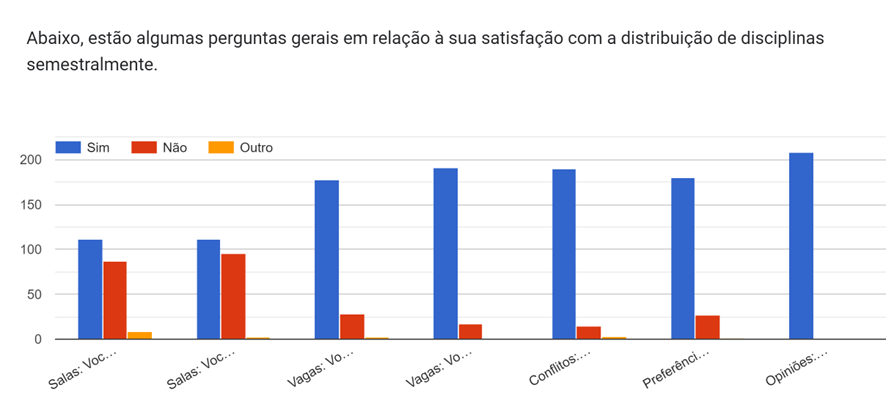
\includegraphics[width=\textwidth]{files/img/2.02!3-organizacao/2.02!3.1.4-forms/3.0-Satisfacao}
\end{MyCenteredFigure} % Satisfacao

Quanto à distribuição dos recursos físicos, vemos uma taxa de 53,1\% de alunos que já tiveram que mudar de sala por falta de algum acessório disposto necessário para a aula. Já a necessidade de mudança de sala devido à ausência de carteiras suficientes obteve taxa de 52,7\%.

É notório o receio dos alunos quanto à possibilidade de não conseguir se inscrever nas disciplinas que desejam cursar, tendo sido confirmado por 85,0\% dos respondentes que se viram em situação em que a disciplina na qual desejavam se matricular não dispunha de vagas o bastante. Essa realidade resulta no temor por semestralmente não conseguir se inscrever na disciplina desejada, fazendo com que 91,3\% dos respondentes tenham se mantido acordados após a meia-noite por causa deste medo.

O temor de não conseguir se inscrever nas disciplinas desejadas é ainda agravado pelo fato de que 90,8\% dos alunos que já deixaram de se inscrever em disciplinas devido a conflitos de horário.

O que se apresenta como um agravante ainda maior na percepção da progressão não sequencial dos alunos é a quantidade de alunos que já preferiram não se inscrever em uma disciplina para cursá-la em outro momento mais oportuno, mesmo que isto signifique um atraso na progressão do curso, sendo seu percentual 86,0\%.

Embora seja uma prática recorrente a oferta de diversas turmas para uma mesma disciplina, o que usualmente é feito de forma que as turmas sejam ofertadas no mesmo horário. Entretanto, os alunos, unanimemente, não se mostram satisfeitos com esta prática, visto que 100\% dos respondentes consideram que a universidade deveria dispor de outros horários para as disciplinas mais demandadas com o intuito de evitar conflitos de horários.

Este resultado é curioso, visto que o temor de não se atrasar em seu progresso e conseguir se inscrever nas disciplinas desejadas, contrasta diretamente com a preferência pessoal de não se inscrever em disciplinas e cursá-las posteriormente, mesmo que isso possa atrasar seu progresso. Entende-se que nem todas as disciplinas, caso não cursadas em seu período esperado, resultarão no atraso da grade, mas ainda assim, a antítese é evidente.

\subsection{Preferências pessoais} % #### 4.4.3. Preferências pessoais

Neste segmento, visa-se entender um pouco melhor o processo decisório dos alunos quanto à escolha das disciplinas que desejam cursar. Primeiro, lhes é indagado quanto à disposição das disciplinas, variando entre disciplinas concentradas em poucos dias ou espalhadas durante a semana (\autoref{fig:4.1-PreferenciasPessoais-Distribuida_Acumulada}) e quanto à preferência de horários, variando entre horários matutinos e vespertinos (\autoref{fig:4.2-PreferenciasPessoais-Manha_Tarde}).

Embora não lide com conflitos, a análise de seus resultados pode auxiliar na escolha de distribuição futura dos usuários do sistema, ao desenvolverem a grade horária, caso desejem considerar as preferências dos estudantes.

\begin{MyCenteredFigure}
  \caption{Preferências por distribuição de disciplinas ao longo da semana}
  \label{fig:4.1-PreferenciasPessoais-Distribuida_Acumulada}
  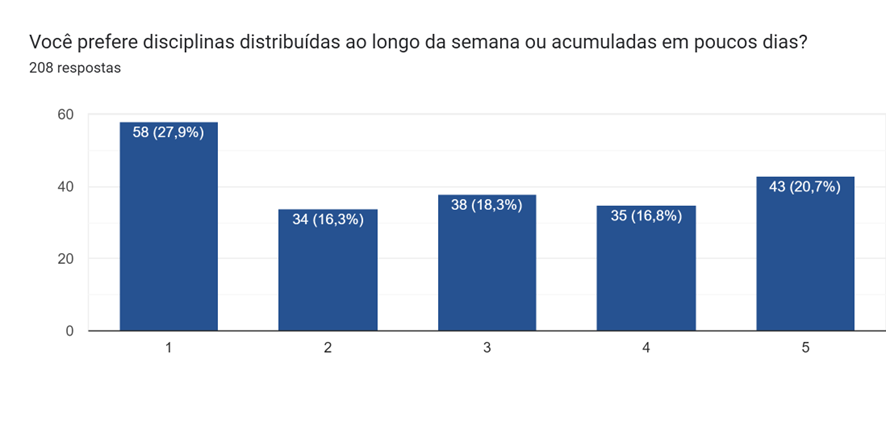
\includegraphics[width=\textwidth]{files/img/2.02!3-organizacao/2.02!3.1.4-forms/4.1-PreferenciasPessoais-Distribuida_Acumulada}
\end{MyCenteredFigure} % PreferenciasPessoais Distribuida_Acumulada

\begin{MyCenteredFigure}
  \caption{Preferências por distribuição de disciplinas em um mesmo dia}
  \label{fig:4.2-PreferenciasPessoais-Manha_Tarde}
  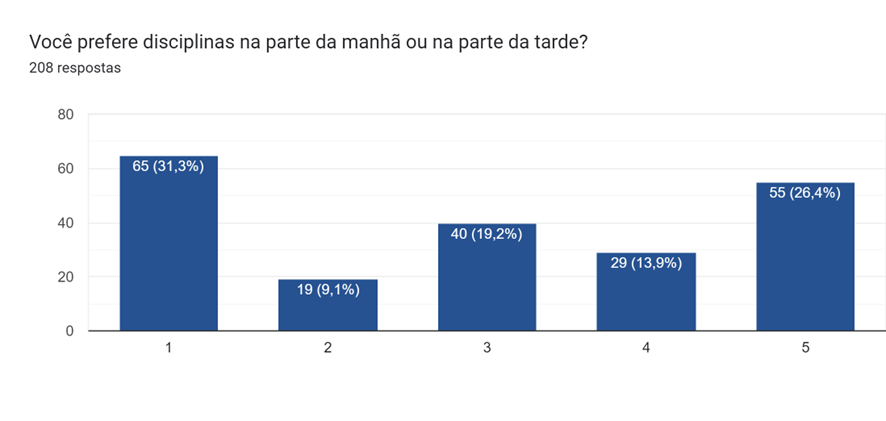
\includegraphics[width=\textwidth]{files/img/2.02!3-organizacao/2.02!3.1.4-forms/4.2-PreferenciasPessoais-Manha_Tarde}
\end{MyCenteredFigure} % PreferenciasPessoais Manha_Tarde

Podemos ver na \autoref{fig:4.1-PreferenciasPessoais-Distribuida_Acumulada} que há uma grande distribuição entre as preferências dos alunos, tendendo às extremidades, onde alguns preferem bastante as disciplinas distribuídas ao longo da semana enquanto outros preferem disciplinas acumuladas em poucos dias, vindo como terceira opção mais votada a neutralidade. Observação similar se mostra presente também na \autoref{fig:4.2-PreferenciasPessoais-Manha_Tarde}.

Como alternativa de visualização, dispomos aqui da \autoref{table:4.1-PreferenciasPessoais-Distribuída_Acumulada} e da \autoref{table:4.2-PreferenciasPessoais-Manha_Tarde} com os resultados numéricos.

\begin{table}[htbp]\centering
  \caption{Preferências por distribuição de disciplinas em um mesmo dia}
  \label{table:4.1-PreferenciasPessoais-Distribuída_Acumulada}
  \begin{tabular}{| r l |}
    \hline
    \textbf{Quantidade} & \textbf{Distribuição na semana} \\
    \hline
    58                  & Distribuídas ao longo da semana \\
    34                  & $\sim$                          \\
    38                  & Não tenho preferência           \\
    35                  & $\sim$                          \\
    42                  & Acumuladas em poucos dias       \\
    \hline
  \end{tabular}
\end{table}

\begin{table}[htbp]\centering
  \caption{Preferências por distribuição de disciplinas em um mesmo dia}
  \label{table:4.2-PreferenciasPessoais-Manha_Tarde}
  \begin{tabular}{| r l |}
    \hline
    \textbf{Quantidade} & \textbf{Distribuição no dia} \\
    \hline
    65                  & Na parte da manhã            \\
    19                  & $\sim$                       \\
    40                  & Não tenho preferência        \\
    28                  & $\sim$                       \\
    55                  & Na parte da tarde            \\
    \hline
  \end{tabular}
\end{table}

Em seguida, é questionado sobre qual é o critério de seleção de disciplinas que se apresentam conflituosas (\autoref{fig:4.3-PreferenciasPessoais-Conflitos}). Nesta vertente vemos uma maior propensão às disciplinas que é pré-requisito de uma grande quantidade de disciplinas, ou seja, disciplinas que, caso se tenham reprovação ou não sejam cursadas, resultam no que é coloquialmente chamado de ``prender disciplinas'', assim atrasando mais a progressão do aluno. Sendo este o critério adotado por 81,3\% dos respondentes. A segunda maior opção selecionada foi a de escolher a disciplina mais concorrida, ou seja, a disciplina que possui uma maior demanda de alunos, sendo um critério utilizado por 25\% dos alunos. Os valores exatos podem ser vistos na \autoref{table:4.3-PreferenciasPessoais-Conflitos}.

\begin{MyCenteredFigure}
  \caption{Critérios para a escolha de disciplinas conflituosas}
  \label{fig:4.3-PreferenciasPessoais-Conflitos}
  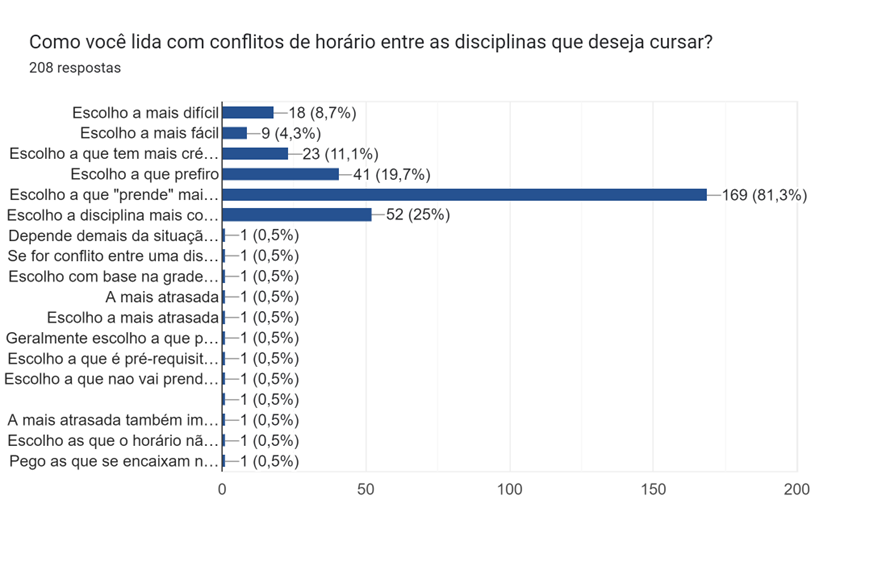
\includegraphics[width=\textwidth]{files/img/2.02!3-organizacao/2.02!3.1.4-forms/4.3-PreferenciasPessoais-Conflitos}
\end{MyCenteredFigure} % PreferenciasPessoais Conflitos

Vale ressaltar que as respostas ilustradas pela \autoref{fig:4.3-PreferenciasPessoais-Conflitos} permite a seleção de múltiplas escolhas, inclusive permitindo que adicionassem outros critérios próprios. Dentre eles, um se mostrou ligeiramente recorrente que seria escolher a disciplina mais atrasada segundo a grade curricular. Outra possibilidade citada foi selecionar a que se encaixam na disponibilidade de horário pessoal, para que não conflite, por exemplo, com o horário do estágio obrigatório.

\begin{table}[htbp]\centering
  \caption{Critérios para a escolha de disciplinas conflituosas}
  \label{table:4.3-PreferenciasPessoais-Conflitos}
  \begin{tabular}{| r l |}
    \hline
    \textbf{Quantidade} & \textbf{Forma de escolher disciplina conflituosa} \\
    \hline
    169                 & Escolho a que ``prende'' mais matérias            \\
    52                  & Escolho a disciplina mais concorrida              \\
    41                  & Escolho a que prefiro                             \\
    23                  & Escolho a que tem mais créditos                   \\
    18                  & Escolho a mais difícil                            \\
    11                  & Outro                                             \\
    9                   & Escolho a mais fácil                              \\
    \hline
  \end{tabular}
\end{table}

\subsection{Experiências com atrasos e disciplinas} % #### 4.4.4. Experiências passadas com atrasos e disciplinas

Quanto aos atrasos para a realização de disciplinas, o ideal desejado é que não haja nenhum atraso. Nessa situação, todos os alunos que entram na universidade poderão seguir a disponibilidade usual das disciplinas dispostas em suas grades curriculares, que apresentam o período esperado para que cada disciplina seja realizada. Sendo elas, usualmente dividas como disciplinas pares e ímpares. As ímpares se referem às disciplinas em que se espera que sejam cursadas nos períodos 1, 3, 5, 7 e 9, e que são ofertadas no primeiro semestre letivo. Enquanto que as pares se referem às disciplinas oferecidas no segundo período letivo, onde geralmente se alocam as disciplinas dos períodos 2, 4, 6, 8 e 10.

Entretanto, a realidade dos alunos é outra. Isso se dá por diversos motivos, seja por reprovação, por não conseguir se inscrever na disciplina desejada ou por simplesmente não ter interesse em cursar a disciplina naquele momento, como já ilustrado na \autoref{fig:3.0_Satisfacao}. Esta característica se confirma na percepção da frequência e distância que percebemos dos atrasos, representado pela \autoref{fig:5.1-Atrasos-Esperar} e pela \autoref{fig:5.2-Atrasos-Distancia}.

\begin{MyCenteredFigure}
  \caption{Períodos de atraso por espera}
  \label{fig:5.1-Atrasos-Esperar}
  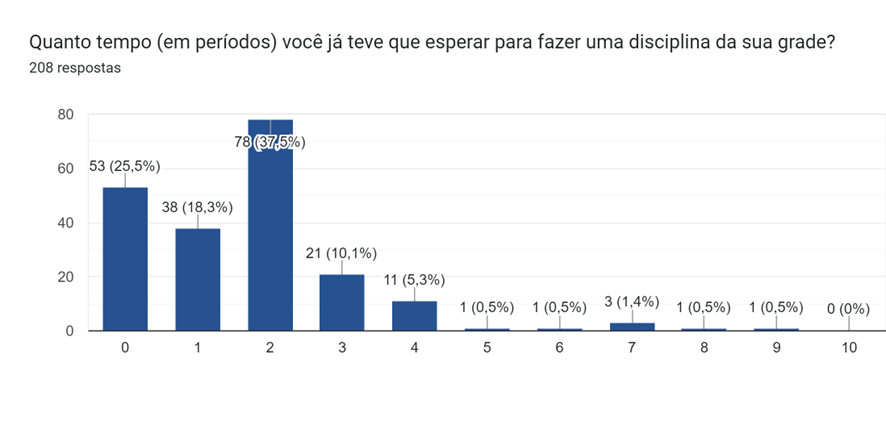
\includegraphics[width=\textwidth]{files/img/2.02!3-organizacao/2.02!3.1.4-forms/5.1-Atrasos-Esperar}
\end{MyCenteredFigure} % Atrasos

\begin{MyCenteredFigure}
  \caption{Distância de atraso}
  \label{fig:5.2-Atrasos-Distancia}
  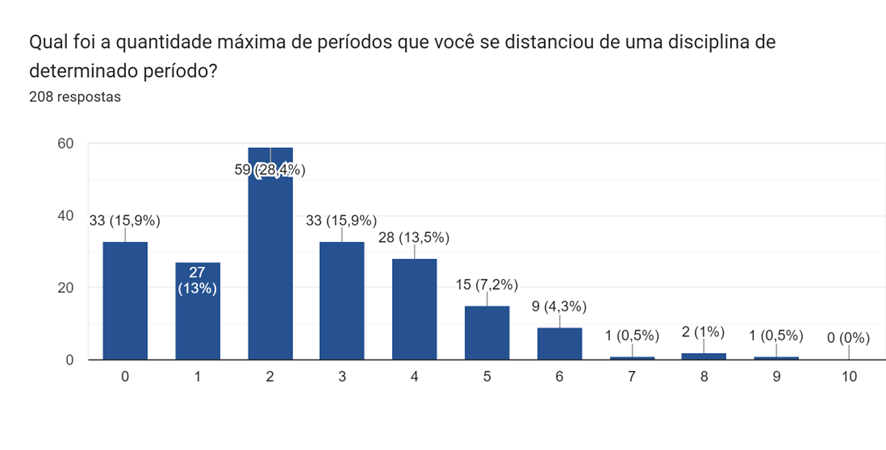
\includegraphics[width=\textwidth]{files/img/2.02!3-organizacao/2.02!3.1.4-forms/5.2-Atrasos-Distancia}
\end{MyCenteredFigure} % Atrasos
Apresenta-se notável que é minoria a quantidade de alunos que nunca tiveram que esperar para cursar uma disciplina, sendo estes apenas 25,5\% dos respondentes. É ainda mais notável o fato de que o tempo de espera médio é de mais de um ano e meio. Quanto ao distanciamento de disciplinas, seja por reprovações ou por escolha própria se mostra ainda mais presente, sendo que apenas 15,9\% dos respondentes não se distanciaram das disciplinas esperadas para o período, sendo 2.8 anos o tempo médio de distanciamento.

Abaixo, encontra-se disposto na \autoref{table:5.0-Atrasos} os resultados obtidos através desta seção do formulário.

\begin{enumerate}
  \item Quanto tempo (em períodos) você já teve que esperar para fazer uma disciplina da sua grade?
  \item Qual foi a quantidade máxima de períodos que você se distanciou de uma disciplina de determinado período?
\end{enumerate}

\begin{table}[htbp]\centering
  \caption{Tempo de atraso em disciplinas}
  \label{table:5.0-Atrasos}
  \begin{tabular}{| c | c c c c c c c c c c c |}
    \hline
    \multicolumn{1}{|c|}{\multirow{2}{*}{Pergunta}} &
    \multicolumn{11}{c|}{Períodos de atraso}                                                          \\
    \multicolumn{1}{|c|}{}                          &
    \multicolumn{1}{c|}{0}                          &
    \multicolumn{1}{c|}{1}                          &
    \multicolumn{1}{c|}{2}                          &
    \multicolumn{1}{c|}{3}                          &
    \multicolumn{1}{c|}{4}                          &
    \multicolumn{1}{c|}{5}                          &
    \multicolumn{1}{c|}{6}                          &
    \multicolumn{1}{c|}{7}                          &
    \multicolumn{1}{c|}{8}                          &
    \multicolumn{1}{c|}{9}                          &
    \multicolumn{1}{|c|}{10}
    \\
    \hline
    1                                               & 53 & 38 & 79 & 19 & 11 & 1  & 1 & 3 & 1 & 1 & 0 \\
    2                                               & 33 & 27 & 60 & 31 & 28 & 15 & 9 & 1 & 2 & 1 & 0 \\
    \hline
  \end{tabular}
\end{table}

\subsection{Pesquisa de opinião} % #### 4.4.5. Opiniões quanto à distribuição das disciplinas

Aqui, buscamos uma análise mais bruta e direta à concordância dos respondentes quanto às características atribuídas à distribuição de disciplinas semestrais, ondem eles avaliam com notas de 1 a 5 o quanto concordam com cada uma das características dadas à distribuição de disciplinas, sendo eles ``Justa'', ``Variada'', ``Contínua'', ``Eficiente'', ``Distribuída'' e ``Satisfatória''. Estando as opiniões dos alunos quanto às três primeiras refletidas nos resultados expostos pela \autoref{fig:6.0-Opiniao-1_3} enquanto que as três últimas são ilustradas pela \autoref{fig:6.0-Opiniao-4_6}.

% \begin{MyCenteredFigure}
% \centering
%    \caption{Notas dadas para as características  da distribuição de disciplinas}
% \label{fig:6.0-Opiniao-Todas}
%    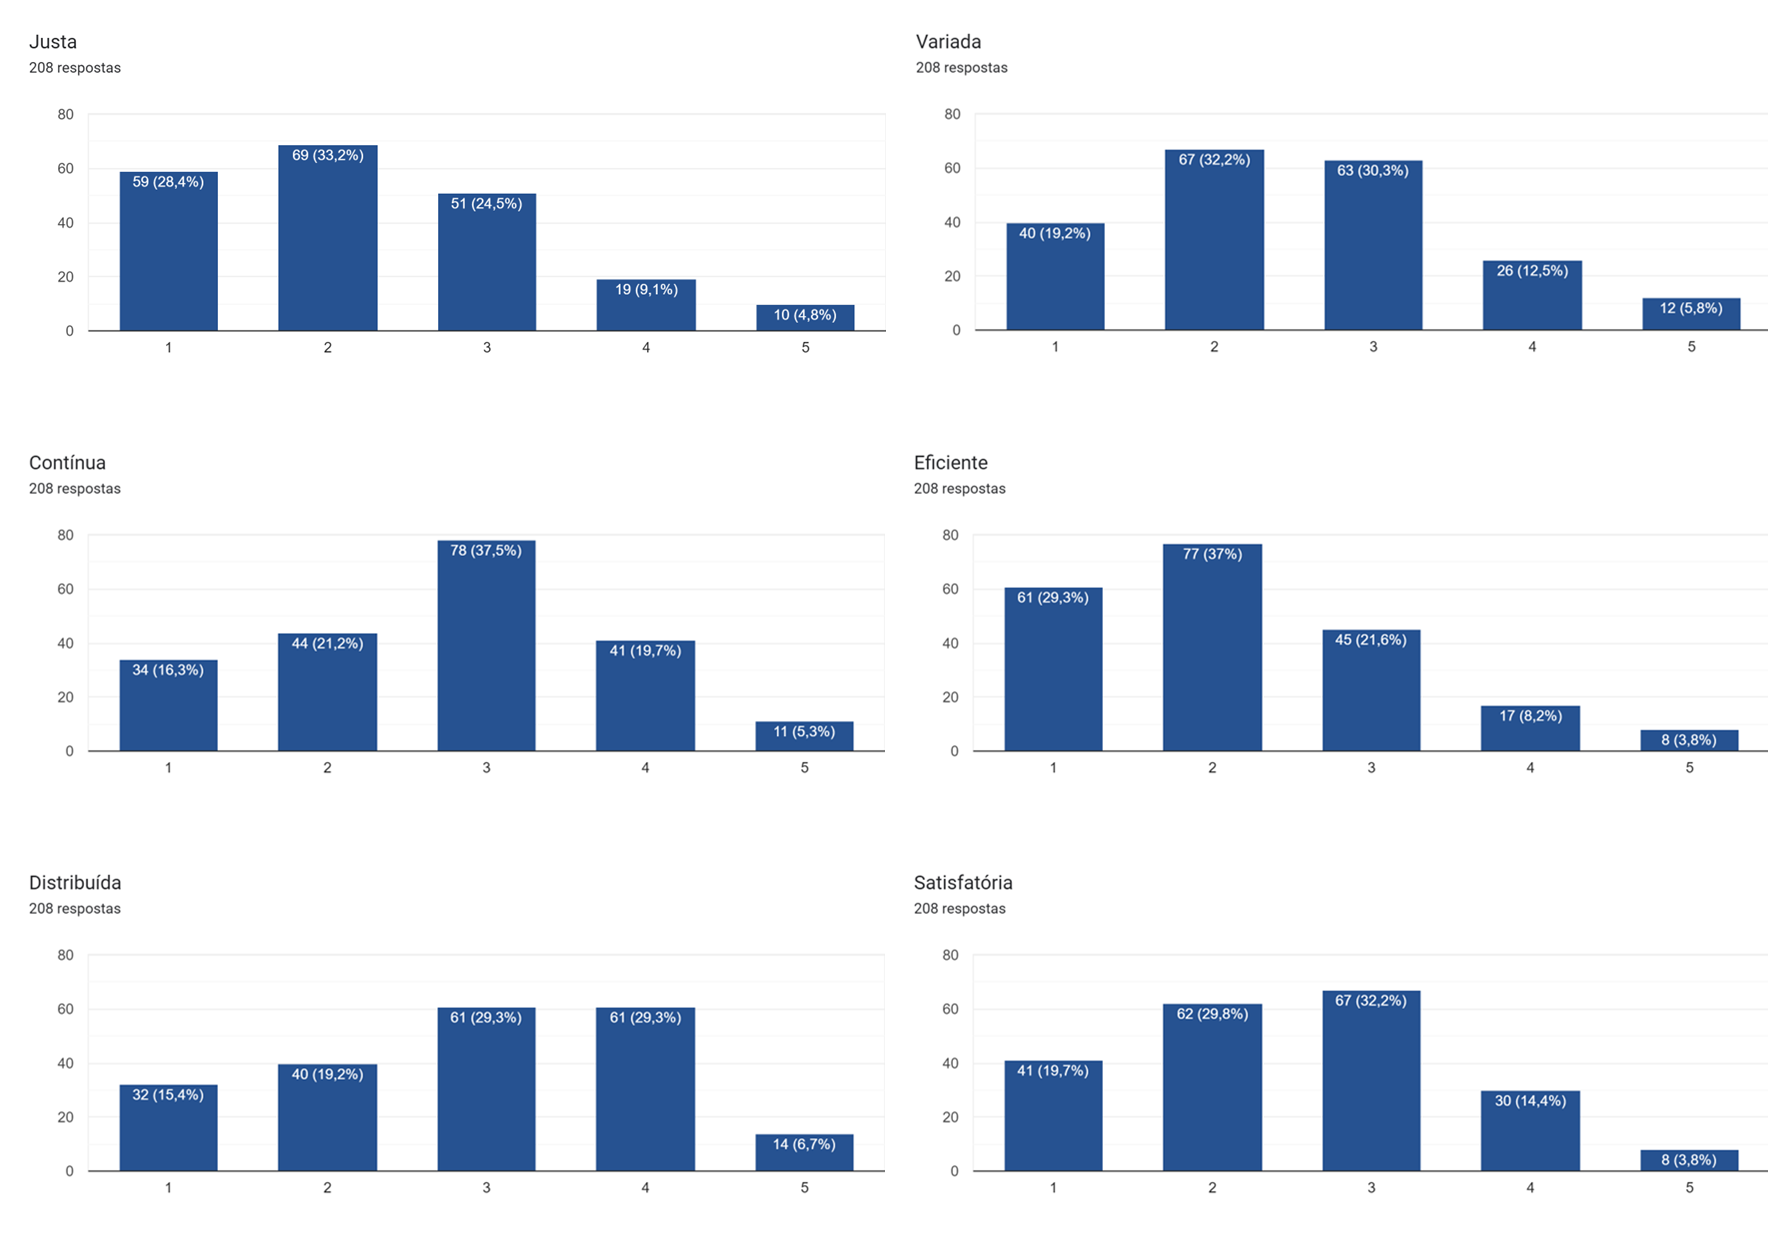
\includegraphics[width=\textwidth]{files/img/2.02!3-organizacao/2.02!3.1.4-forms/6.0-Opiniao-Todas}
% \end{MyCenteredFigure}

\begin{MyCenteredFigure}
  \caption{Notas dadas para as características ``Justa'', ``Variada'' e ``Contínua''}
  \label{fig:6.0-Opiniao-1_3}
  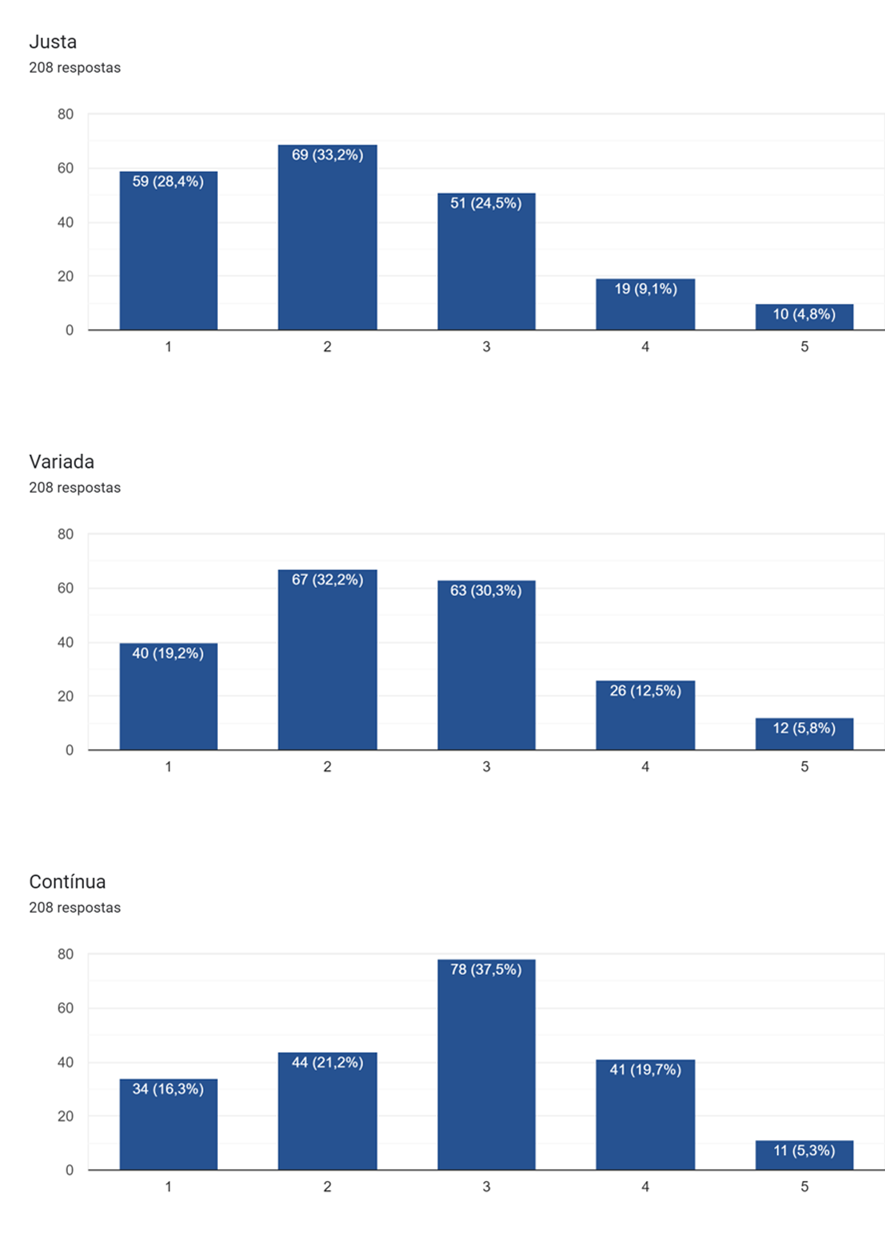
\includegraphics[width=\textwidth]{files/img/2.02!3-organizacao/2.02!3.1.4-forms/6.0-Opiniao-1_3}
\end{MyCenteredFigure}

\begin{MyCenteredFigure}
  \caption{Notas dadas para as características ``Eficiente'', ``Distribuída'' e ``Satisfatória''}
  \label{fig:6.0-Opiniao-4_6}
  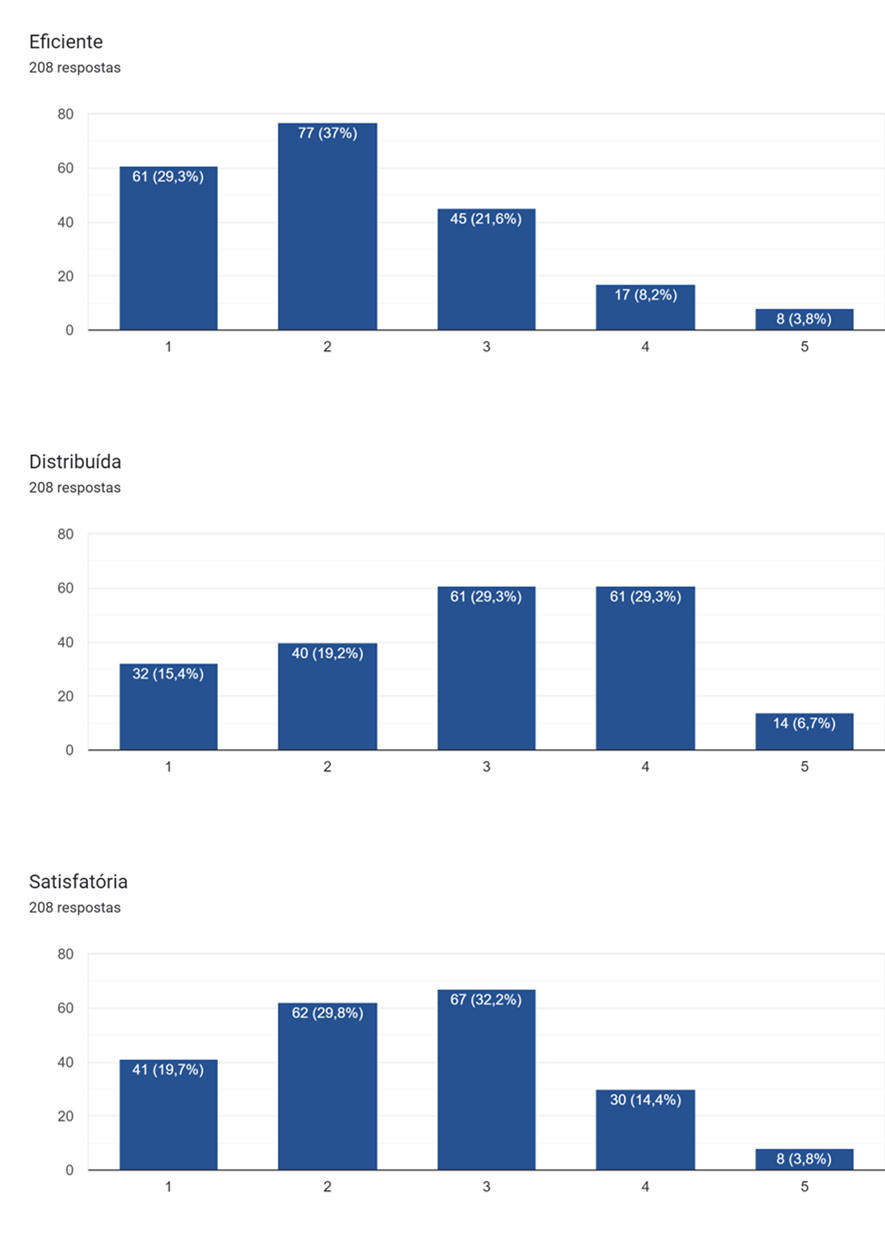
\includegraphics[width=\textwidth]{files/img/2.02!3-organizacao/2.02!3.1.4-forms/6.0-Opiniao-4_6}
\end{MyCenteredFigure}

% \begin{MyCenteredFigure}
%    \caption{Notas dadas para a característica: justa}
%    \label{fig:6.1-Opiniao-Justa}
%    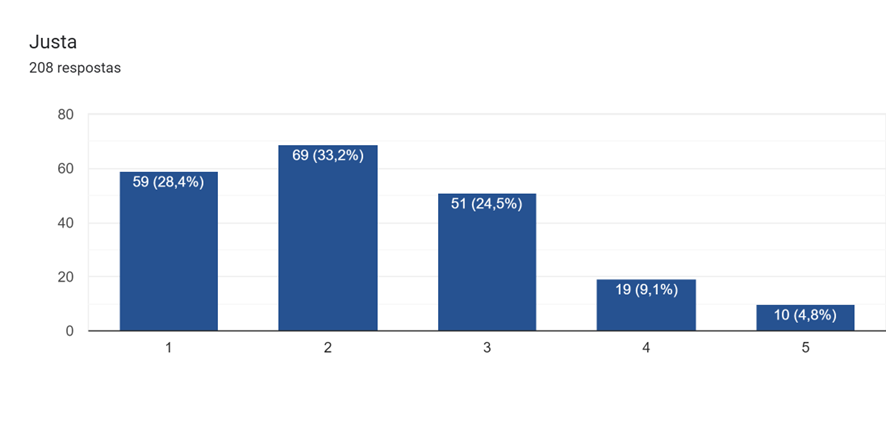
\includegraphics[width=\textwidth]{files/img/2.02!3-organizacao/2.02!3.1.4-forms/6.1-Opiniao-Justa}
% \end{MyCenteredFigure} % Opiniao-Justa

% \begin{MyCenteredFigure}
%    \caption{Notas dadas para a característica: variada}
%    \label{fig:6.2-Opiniao-Variada}
%    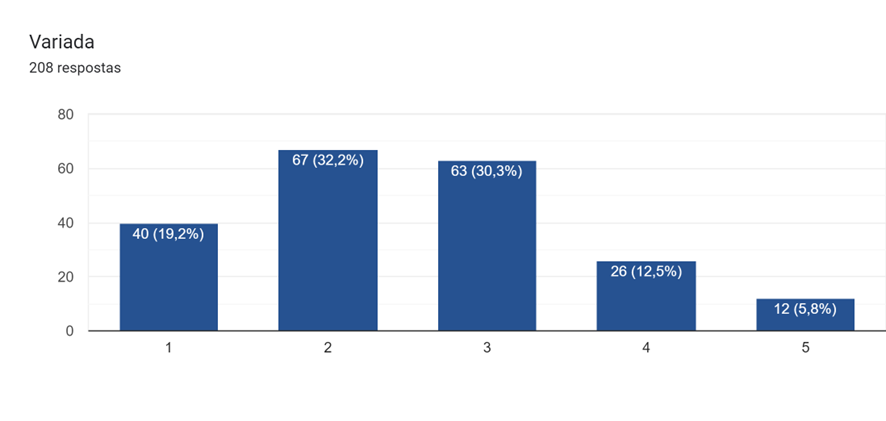
\includegraphics[width=\textwidth]{files/img/2.02!3-organizacao/2.02!3.1.4-forms/6.2-Opiniao-Variada}
% \end{MyCenteredFigure} % Opiniao-Variada

% \begin{MyCenteredFigure}
%    \caption{Notas dadas para a característica: contínua}
%    \label{fig:6.3-Opiniao-Continua}
%    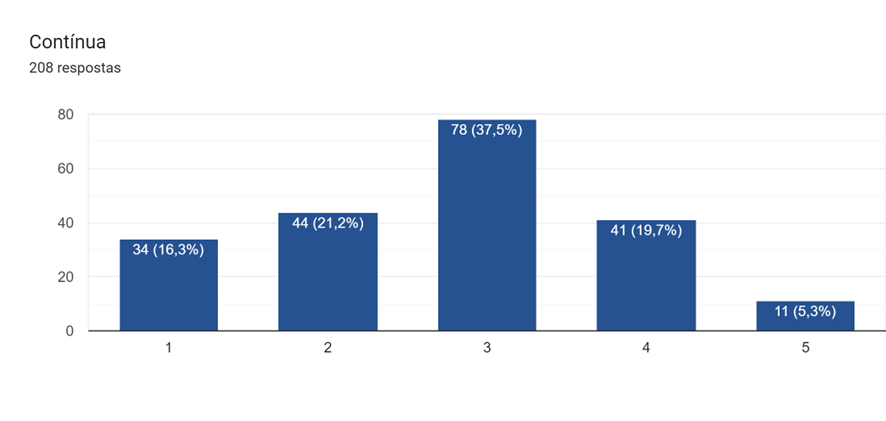
\includegraphics[width=\textwidth]{files/img/2.02!3-organizacao/2.02!3.1.4-forms/6.3-Opiniao-Continua}
% \end{MyCenteredFigure} % Opiniao-Continua

% \begin{MyCenteredFigure}
%    \caption{Notas dadas para a característica: eficiente}
%    \label{fig:6.4-Opiniao-Eficiente}
%    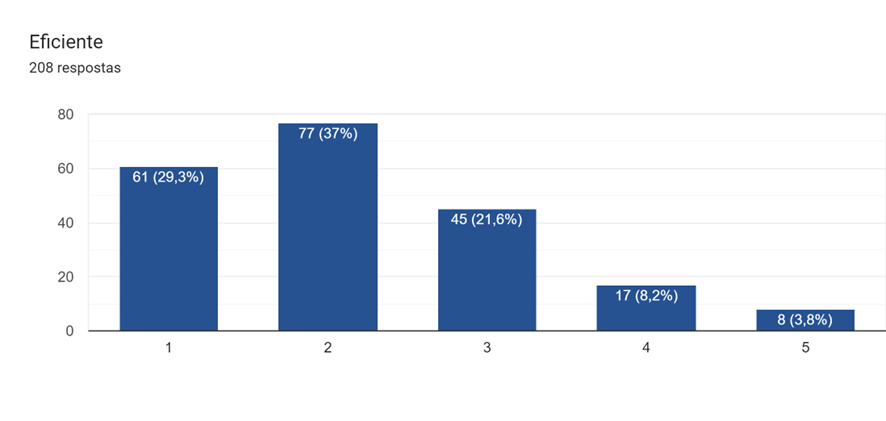
\includegraphics[width=\textwidth]{files/img/2.02!3-organizacao/2.02!3.1.4-forms/6.4-Opiniao-Eficiente}
% \end{MyCenteredFigure} % Opiniao-Eficiente

% \begin{MyCenteredFigure}
%    \caption{Notas dadas para a característica: distribuída}
%    \label{fig:6.5-Opiniao-Distribuida}
%    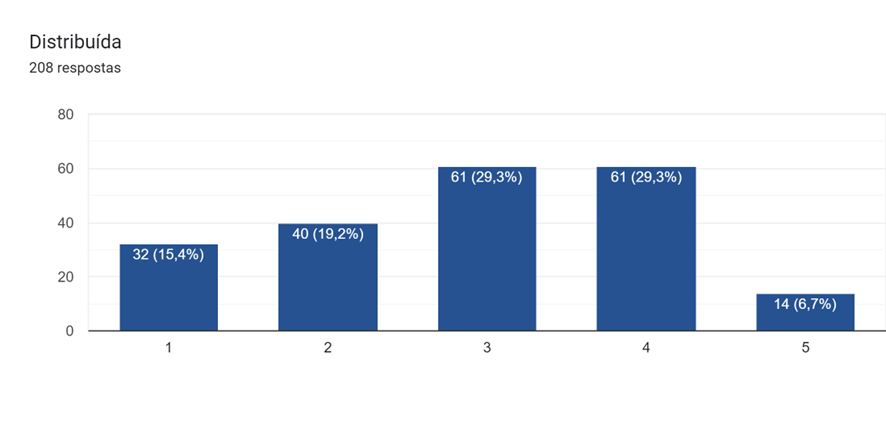
\includegraphics[width=\textwidth]{files/img/2.02!3-organizacao/2.02!3.1.4-forms/6.5-Opiniao-Distribuida}
% \end{MyCenteredFigure} % Opiniao-Distribuida

% \begin{MyCenteredFigure}
%    \caption{Notas dadas para a característica: satisfatória}
%    \label{fig:6.6-Opiniao-Satisfatoria}
%    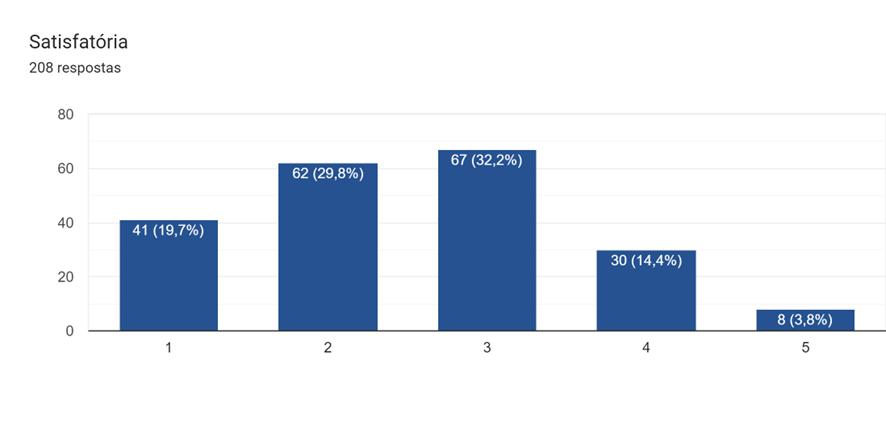
\includegraphics[width=\textwidth]{files/img/2.02!3-organizacao/2.02!3.1.4-forms/6.6-Opiniao-Satisfatoria}
% \end{MyCenteredFigure} % Opiniao-Satisfatoria

De uma forma geral, conseguimos ver todos os gráficos com menos de 7\% dos respondentes dando nota 5 em cada uma das características, A maioria das respostas tende a estar entre 1 e 3, sendo exceção apenas no caso da característica ``distribuída'', que por sua vez apresenta uma elevada quantidade de notas 4, sendo referente a 29,3\% dos respondentes.

Como forma tabular, temos, na \autoref{table:6.0-Opiniao}, as respostas dos alunos, seguidas das médias por característica.

\begin{table}[htbp]\centering
  \caption{Notas dadas às características da distribuição de disciplinas}
  \label{table:6.0-Opiniao}
  \begin{tabular}{| l | c c c c c | c |}
    \hline
    \multicolumn{1}{|c|}{\multirow{2}{*}{Opções}} &
    \multicolumn{5}{c|}{Notas}                    &
    \multicolumn{1}{|c|}{\multirow{2}{*}{Médias}}
    \\
    \multicolumn{1}{|c|}{}                        &
    \multicolumn{1}{c|}{1}                        &
    \multicolumn{1}{c|}{2}                        &
    \multicolumn{1}{c|}{3}                        &
    \multicolumn{1}{c|}{4}                        &
    \multicolumn{1}{c|}{5}                        &
    \multicolumn{1}{|c|}{}                                                       \\
    \hline
    Justa                                         & 59 & 69 & 52 & 17 & 10 & 2,3 \\
    Variada                                       & 40 & 65 & 64 & 26 & 12 & 2,5 \\
    Contínua                                      & 34 & 44 & 78 & 41 & 10 & 2,8 \\
    Eficiente                                     & 61 & 76 & 45 & 17 & 8  & 2,2 \\
    Distribuída                                   & 32 & 40 & 61 & 60 & 14 & 2,9 \\
    Satisfatória                                  & 40 & 61 & 68 & 30 & 8  & 2,5 \\
    \hline
  \end{tabular}
\end{table}

Ao analisarmos a média de cada uma, podemos dizer que, em suma, há o visível desagrado do corpo discente quanto à distribuição de disciplinas semestrais, com ênfase nas duas piores notas que são 2,2 para ``eficiente'' e 2,3 para ``justa'' o que reforça a necessidade de aprimoramento do sistema atual.

\subsection{Respostas qualitativas} % #### 4.4.6. Respostas qualitativas

Por fim, havia um espaço livre no formulário para que os alunos pudessem expressar suas opiniões de forma mais livre. Após a leitura de todas e a filtragem das opiniões expressas, resumem-se em 4 parabenizações pelo desenvolvimento do presente projeto, 18 reclamações e 16 sugestões. Dentre elas, algumas apresentaram maior recorrência, sendo elas:

\begin{itemize}
  \item 5 reclamações sobre a usual oferta de disciplinas separadas entre pares e ímpares;
  \item 4 reclamações sobre o Sistema Acadêmico, principalmente sobre não ser capaz de suportar a carga nos momentos iniciais de inscrição de disciplinas;
  \item 3 sugestões de ofertas de disciplinas recorrentemente, com ênfase nas disciplinas de matemática/que contemplam diversos cursos/com alta taxa de reprovação;
  \item 3 sugestões de mais oferta de disciplinas no período de verão;
  \item 2 sugestões de que inscrições em matérias do semestre atual esperado do aluno fossem feitas automaticamente, mas ainda permitindo a sua exclusão caso desejado;
  \item 1 sugestão de criação de um formulário de demanda no acadêmico que computasse a intenção de matrícula dos alunos.
\end{itemize}

Abaixo estão dispostas algumas das respostas obtidas:

\begin{itemize}
  \item ``A estrutura curricular deveria ser predefinida, automatizando a matrícula dos alunos nas disciplinas correspondentes aos seus períodos acadêmicos. No entanto, permitir-se-ia a edição do cronograma por parte dos alunos, caso desejem quitar pendências de períodos anteriores ou disciplinas antecipadas. Além disso, disciplinas que abrangem múltiplos cursos devem ser oferecidas em ambos os semestres.

        Para melhorar a oferta de disciplinas, seria aconselhável ampliar a disponibilidade de disciplinas durante o período de verão. Isso facilitaria o acesso dos alunos ao estágio obrigatório durante as férias, viabilizando a conclusão dessa etapa essencial do curso. Reduzir o número de créditos necessários para antecipar a realização do estágio também se mostraria benéfico, visto que atualmente, a conclusão dessa matéria com apenas 9 créditos pendentes inviabiliza a possibilidade de antecipação antes do 9º período. Considera-se viável permitir essa antecipação a partir do 7º período.

        [...]
        Essas melhorias no sistema acadêmico [...] agilizariam a trajetória do estudante, permitindo maior flexibilidade na escolha e realização de disciplinas [...].''
  \item ``Existe muita desorganização em relação a grade, disciplinas e sistema acadêmico por parte dos coordenadores dos cursos. Me inscrevi numa matéria que tinha requisito de acordo com o plano pedagógico, mas tanto na grade como no sistema acadêmico não tinha pré-requisito nenhum. Tive que desistir da matéria pela dificuldade, até porque a matéria que era pré-requisito eu perdi. Detalhe: Outras pessoas perderam na matéria pré-requisito e continuaram fazendo a matéria desse período.''
  \item ``Acho que as coordenações precisam estabelecer um melhor diálogo com os alunos. Esse sistema de período par e Ímpar na UENF é antigo e perpetua um comodismo dos professores que acabam não ofertando disciplinas todos os semestres e prejudicando os alunos nas escolhas de matérias optativas, eletivas, instrumentais e obrigatórias tendo que esperar um ano para realizar a disciplina caso você não consiga fazer por choque de horário e/ou reprovação.''
\end{itemize}

\subsection{Conclusões} % #### 4.4.7. Conclusões

Por fim, entendemos que, além das insatisfações dormentes por parte dos gestores e criadores de grades horárias, os alunos também se mostram insatisfeitos com a atual estrutura de distribuição de disciplinas semestrais. Os interesses dos alunos se mostram em sua maioria alinhados com os interesses dos gestores, onde ambos visam reduzir a quantidade de atrasos na progressão do curso.

\section{Exemplo de erros humanos} % contém as imagens que estavan o cap 1

Dada a grande quantidade de variáveis interconectadas e as características específicas de cada instituição \cite{miranda_udpskeduler_2012}, a organização destas informações buscando a melhor solução possível apresenta-se como um desafio. Principalmente se considerarmos que esta solução é, muitas vezes, buscada manualmente, estando também passível de erros humanos como ilustram a \autoref{fig:Academico} e \autoref{fig:CCT}.

\begin{MyCenteredFigure}
  \caption{Disciplina atribuída no sistema acadêmico à determinada hora e local}
  \label{fig:Academico}
  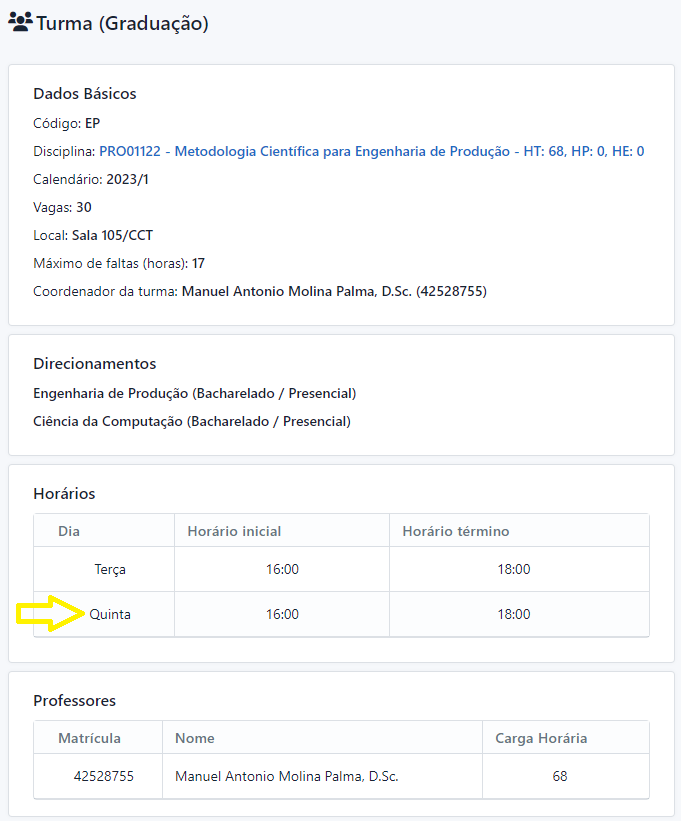
\includegraphics[width=\textwidth]{files/img/2.02!3-organizacao/2.02!3.1.5-erros/Metodologia-Quinta}
\end{MyCenteredFigure}    % Imagem acadêmico

\begin{MyCenteredFigure}
  \caption{Disciplina não atribuída à determinada hora e local na grade de horários do CCT}
  \label{fig:CCT}
  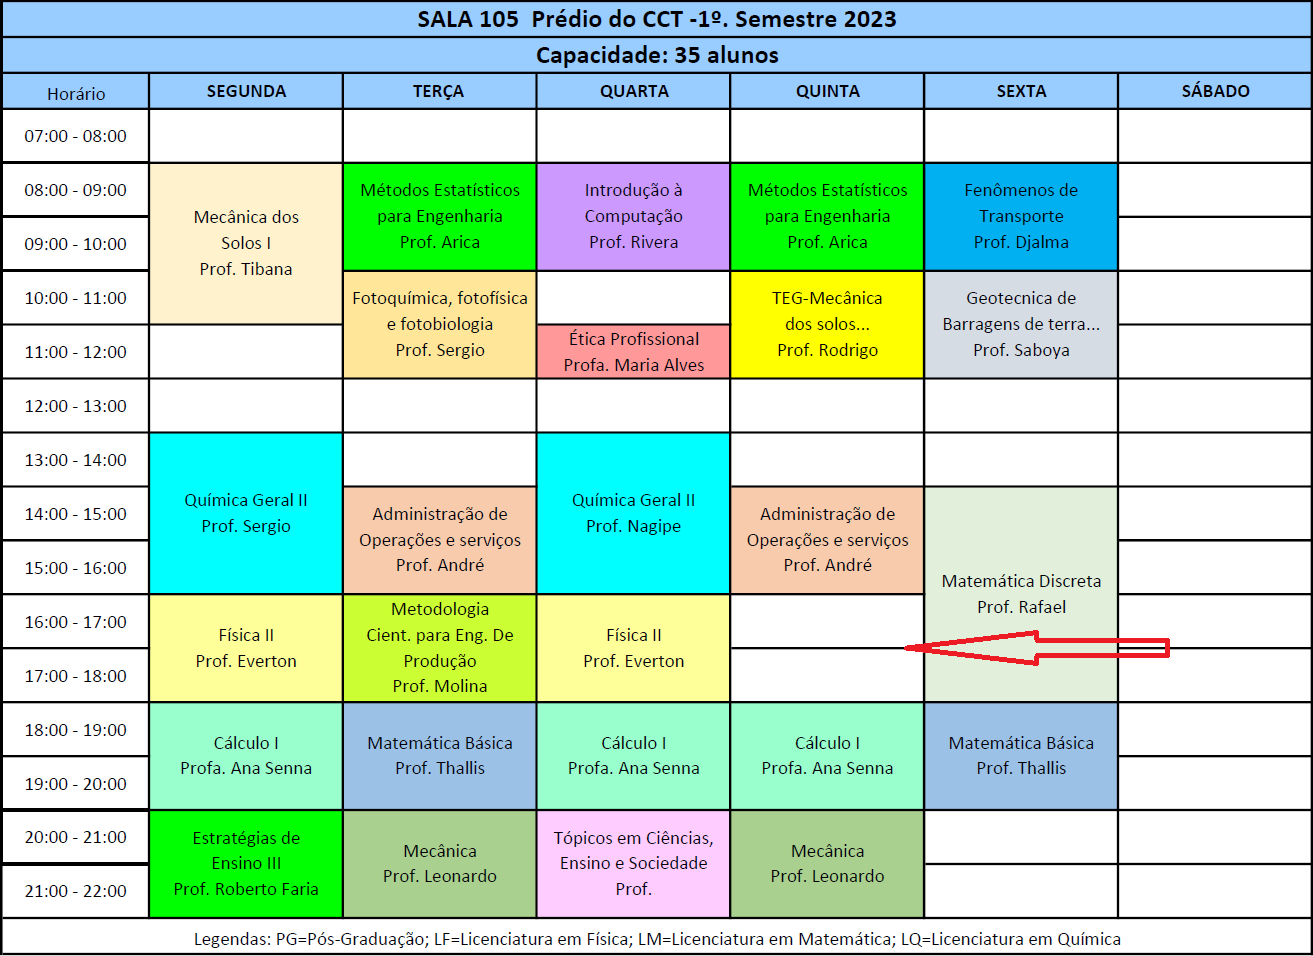
\includegraphics[width=\textwidth]{files/img/2.02!3-organizacao/2.02!3.1.5-erros/Aulas-CCT-105-2023_1}
\end{MyCenteredFigure}    % Imagem representando o erro humano na alocação de salas

Nestas imagens, fica exemplificado um dos possíveis problemas que podem ocorrer durante a criação de grades horárias, que é, mesmo quando uma seção da universidade (o Sistema Acadêmico, ilustrado pela \autoref{fig:Academico}) aloca uma turma a uma determinada sala, outra seção da mesma instituição (o Centro de Ciência e Tecnologia, ilustrado pela \autoref{fig:CCT}) pode não estar ciente do mesmo, ou mesmo estando ciente pode acabar não delimitando aquela lacuna de tempo como ocupada, assim estando passível de uma segunda alocação naquele período de tempo naquela sala, assim gerando problemas.

\section{Relações entre as variáveis} % Mudar o nome da seção depois

A criação de grades horárias é um problema complexo, que envolve uma grande quantidade de variáveis interconectadas. Dentre elas temos as disciplinas, professores, salas, laboratórios, blocos, centros, cursos, alunos, entre outros.

Esta seção visa a análise das relações entre estas variáveis, buscando entender como elas se relacionam e como estas relações podem ser utilizadas para a criação de uma grade horária mais eficiente.

\subsection{Turmas}

As turmas são a base da grade horária, sendo ela a representação da união entre professor, disciplina, alunos, horário e sala. A turma é a representação da oferta de uma disciplina em um determinado horário e local, com um determinado professor e para um determinado grupo de alunos. A turma é a unidade básica da grade horária, e é a partir dela que a grade é construída.

\subsection{Laboratórios}

Os laboratórios são estruturas organizacionais que englobam professores, disciplinas e cursos. Em sua maioria, os laboratórios estão associados a um único curso, entretanto, existem casos em que um laboratório está associado a mais de um curso, como é o caso do LCMAT, que está associado aos cursos de Matemática e de Ciência da Computação.

%- Laboratório percente aos centros
% - Geralmente (o normal é que) cada laboratório tem um único curso
% - LCMAT é o único laboratório que tem dois cursos associados
% - Mas existem vários laboratórios que alimentam um único curso
% - O curso tá associado a 1:n laboratórios
% - O laboratório tá associado a 1:n cursos

\subsection{Professores}

%- Professor pertence ao laboratório
% - Tang: professor do LCMAT

\subsection{Centros}

\subsection{Salas}

\subsection{Cursos}

\subsection{Alunos}

\subsection{Disciplinas} % #### 4.5.1. Disciplinas

Um dos pontos principais na criação de uma grade horária é a alocação das disciplinas. As disciplinas são a base da grade horária,

%- disciplina
% - A disciplina é oferecida pelos laboratórios
% - o curso tem aquela disciplina na grade
% - A disciplina pode ser demandada por 1:n cursos
% - As disciplinas tem as siglas INF de cc/informática e MAT de matemática
% - as siglas das disciplinas são por laboratório, ou em casos específicos, são do centro, CCT/CCH, etc

\subsection{Blocos}

%- Físico
% - Blocos contém salas
% - Salas são administradas por centros
% - Centros não estão limitados por blocos

\subsection{Pactos Sociais}

%- Pactos sociais
% - São entendidos que certas salas têm por padrão uma certa preferência por certos cursos
% - Assim como as disciplinas também são usualmente designadas aos mesmos professores historicamentes
